\documentclass[a4paper,12pt]{article}
\usepackage[francais]{babel} % Package babel pour le français
\usepackage[T1]{fontenc}    % Package pour les accentuations
\usepackage[utf8]{inputenc}  % Français
\usepackage{textcomp}
\usepackage{lmodern}        % Pour avoir de bonnes polices en pdf
\usepackage{graphicx}       % Indispensable pour les figures
\usepackage{epstopdf}       % Utile pour les figures, résout une erreur
\usepackage{amsmath}        % Environnement pour les maths, permet du mettre du texte dans les équations
\usepackage{dialogue}		% Pour les dialogues
\usepackage{geometry}       % Utilisé pour les marges
\usepackage{pst-tree}		% Pour dessiner des arbres
\usepackage{pst-node}
\usepackage{multicol}		% Pour les colonnes
\usepackage{mathtools, bm}  % Typographie pour les ensembles communs
\usepackage{amssymb, bm}    % Typographie pour les ensembles communs
\usepackage{float}          % Pour bien placer les figures, scripts et tableaux
%\usepackage{listings}       % Utilisé pour les scripts
\usepackage{wrapfig}
\usepackage{xcolor}
\usepackage[french,onelanguage,ruled,vlined]{algorithm2e} %Pour les algorithmes
\definecolor{vertclair}{rgb}{0.10,0.55,0.17}
\definecolor{vertfonce}{rgb}{0,0.44,0}
\definecolor{grisclair}{rgb}{0.78,0.78,0.78}
\definecolor{prune}{rgb}{0.65,0.00,0.00}
\definecolor{bleufonce}{rgb}{0.06,0.06,1.00}
\definecolor{violet}{rgb}{0.21,0.18,0.73}
\definecolor{orange}{rgb}{0.93,0.46,0.00}

\usepackage{tikz}			%Pour les figures et graphes
\usetikzlibrary{calc}		%Pour les figures et graphes
\usepackage[cache=false]{minted}        % Utilisé pour les scripts
\geometry{hmargin=2cm,vmargin=2cm} % Réglages des marges
\usepackage{fancyhdr}		% Pour l'entête et les pieds de page
\pagestyle{fancy}			% Pour l'entête et les pieds de page
\usepackage{hyperref}		% Pour les liens hypertext, sommaire et références
\usepackage[final]{pdfpages} % Pour inclure des .pdf

\renewcommand{\abstractname}{Avant-propos} %Modification du titre de l'abstract
\newcommand{\norme}[1]{\left\Vert #1\right\Vert} %Commande pour la norme euclidienne
\renewcommand{\listoflistingscaption}{Liste des programmes} %Pour changer le titre de la liste des codes
\renewcommand{\listingscaption}{Programme} %Pour changer la légende des codes

\SetKwRepeat{doWhile}{faire}{tant que} % Pour les do-while


\newminted{console}{mathescape,

               breaklines = true,
               numbersep=5pt,
               frame=lines,
               framesep=2mm}

\newminted{lisp}{mathescape,

               breaklines = true,
               numbersep=5pt,
               frame=lines,
               framesep=2mm}

\renewcommand{\headrulewidth}{0.5pt}
\fancyhead[L]{IA01}
\fancyhead[R]{TP03 : Réalisation d’un système expert d’ordre $0+$}


\begin{document}


\thispagestyle{empty}

{\large

\vspace*{1cm}

\begin{center}

	{\bf Rapport de IA01 : \\Intelligence artificielle -- Représentation des connaissances}
	\vspace*{1cm}
	{\bf \\UNIVERSITE DE TECHNOLOGIE DE COMPIEGNE}

	\vspace*{1cm}
	
\includegraphics[scale=0.6]{UTC_logo.png}
	\vspace*{1cm}

	Automne 2016

	\vspace*{1cm}

	\vspace*{1cm}
	{\Large {\bf Guillaume JOUNEL \& Julien JERPHANION}}

	\vspace*{2 cm}
\end{center}

\flushleft{Sujet du rapport:\ \\
{\Large {\bf TP03 : Réalisation d’un système expert d’ordre $0+$}}}

\vspace*{1 cm}
\flushleft{Département des étudiants :\ \\
{\Large {\bf  Génie Informatique}}}\\

\vspace*{1 cm}
\flushleft{Professeur :\ \\
{\Large {\bf Marie-Hélène ABEL}}}\\
}

\newpage
\tableofcontents
%\newpage
%\listoffigures
\newpage
\listoflistings
\newpage

\section{Introduction : Présentation du système expert}


\subsection{Problématique}

Tous les programmeurs sont un jour confrontés au problème suivant :

\begin{quotation}
\centering
« \textit{Quels de programmation et technologies sont les plus adaptés pour le projet que je souhaite développer dans mon cadre d'utilisation ?} »

\end{quotation}


    Pour pallier à ce problème, nous allons concevoir un système expert qui propose différentes possibilités les plus adaptées selon l'usage.

    Pour cela, nous prendrons en compte de multiples critères tels que le besoin (traiter de l'information, découvrir des concepts informatiques...), ou encore les caractéristiques de sa machine (Linux, MacOS...).

\subsection{Sources de connaissances sur le sujet}

    Les sources d'expertise ne manquent pas : il existe de nombreux sites et ressources sur le Net qui donnent les avantages et inconvénients de toutes les technologies existantes selon les cas d'utilisation. En voici quelques uns :
    \begin{itemize}
        \item Wikipédia : Liste des langages de programmations par type :\\ \href{https://en.wikipedia.org/wiki/List_of_programming_languages_by_type}{\texttt{https://en.wikipedia.org/wiki/List\_of\_programming\_languages\_by\_type}} ;
        \item Learneroo: The Different Programming Languages :\\ \href{https://www.learneroo.com/modules/12/nodes/94}{\texttt{https://www.learneroo.com/modules/12/nodes/94}} ;
        \item WhoIsHostingThis: What Code Should You Learn?\\ \href{http://www.whoishostingthis.com/blog/2014/09/04/learn-to-code/}{\texttt{http://www.whoishostingthis.com/blog/2014/09/04/learn-to-code/}}.
    \end{itemize}

	En tant qu'étudiants ingénieurs en informatique, nous avons aussi sollicité certaines de nos connaissances dans le domaine.

\section{Architecture}

\subsection{Rappels sur l'architecture}
Rappelons rapidement l'architecture d'un système expert.
Un système expert est constitué de trois parties principales dissociées les unes des autres : une \textit{base de faits}, une \textit{base de règles}, et un \textit{moteur d'inférence}.\\

La base de faits est une base d'informations qui comprend les faits initiaux et déduits au cours du programme.\\

La base de règles contient les différentes règles (connaissances implicites de l'expert rendues explicites pour être représentées informatiquement) utilisées pour déduire d'autres faits.\\

Les inférences au cours du processus sont réalisées par le moteur d'inférence. C'est lui qui fait le lien entre les deux précédentes bases. Il exécute les règles contenues dans la base de règles au regard des faits présents dans la base de faits ; les règles étant déclenchables en fonction des faits avérés. À la fin de l'exécution d'une règle, le résultat retourné qui est aussi un fait est stocké dans la base de faits.\\

Il existe deux types de fonctionnement pour les moteurs d'inférence : le \textit{chaînage avant} et le \textit{chaînage arrière}.

Le chaînage avant consiste à regarder les faits présents et à choisir une règle qui peut être exécutée : on cherche les résultats que l'on peut obtenir en se basant sur les résultats déjà obtenus.

Le chaînage arrière examine les règles à exécuter pour arriver à un certain fait : on cherche un moyen d'arriver à un certain résultat.


	Il s'agit ici de construire un système expert d'ordre $0+$ -- que nous avons choisi d'appeler \textit{Cactus} --, c'est à dire un système expert manipulant des faits qui ne sont non pas des propositions booléennes mais des \textit{triplets} comportant trois parties :
	\begin{enumerate}
		\item un attribut, qui est le nom du concept que l'on veut modéliser dans le fait ;
		\item une valeur, qui permet de quantifier l'attribut ;
		\item un opérateur, qui permet de préciser la valeur de l'attribut
	\end{enumerate}
	
	Ainsi \mintinline{lisp}{(temperature >= 30)} et \mintinline{lisp}{(saison EQ été)} sont des faits vus sous l'angle d'un système-expert d'ordre $0+$ dont les attributs, les opérateurs et les valeurs sont respectivement 	\mintinline{lisp}{temperature} et \mintinline{lisp}{saison}, \mintinline{lisp}{>=} et \mintinline{lisp}{EQ}, et \mintinline{lisp}{30} et \mintinline{lisp}{été}.

\subsection{Base de faits}

Puisqu'il s'agit de concevoir un système expert d'ordre $0+$, nous avons choisi d'implémenter nos faits selon la forme suivante :

\begin{quotation}
	\mintinline{lisp}{(attribut EQ valeur)}
\end{quotation}

La base de faits est stockée dans une variable globale \mintinline{lisp}{*faits*} initialement vide : elle se remplira au cours de l'exécution du système. Il s'agira d'une liste de triplets.\\

Voici quelques exemples d'attributs que nous utiliserons pour modéliser les faits :

\begin{table}[H]
		\label{exempleAttributs}
		\centering{
    		\begin{tabular}{|l|c|}
    		\hline
    		Attributs & Signification\\
    		\hline
    		\hline
    		\mintinline{lisp}{UserStory} & scénario initial de l'utilisateur \\
    		\mintinline{lisp}{Application} & le type d'application à développer  \\
    		\mintinline{lisp}{Machine} & le type d'OS utilisé pour développer \\
    		\mintinline{lisp}{Cible} & le type d'OS visé pour l'application \\
    		\mintinline{lisp}{Budget} & le budget du développeur \\
    		\mintinline{lisp}{Paradigme} & précise le paradigme des bases de données\\
    		\hline
		\end{tabular}}
		\caption{Exemple d'attributs pour les faits}
\end{table}

\mintinline{lisp}{Propositions} sera l'attribut du faits utilisé pour stocker les différentes propositions inférées par \textit{Cactus}.

\subsection{Base de règles}
Nous avons décidé d'implémenter les règles dans notre base de cette façon :

\begin{minted}{lisp}
	(((Premisse1 operateur valeur)...(PremisseN operateur valeur))
  	  ((Resultat1 operateur valeur)...(Resultat1M operateur valeur)))
\end{minted}
où $\mintinline{lisp}{operateur} \in \{\mintinline{lisp}{=},\mintinline{lisp}{<},\mintinline{lisp}{>},\mintinline{lisp}{EQ}\} $.
\begin{listing}[H]
	\centering
	\inputminted[breaklines=true,linenos,lastline=43]{lisp}{../regles.lisp}
\end{listing}

\begin{listing}[H]
	\centering
	\inputminted[breaklines=true,linenos,firstline=44,lastline=88]{lisp}{../regles.lisp}
\end{listing}

\begin{listing}[H]
	\centering
	\inputminted[breaklines=true,linenos,firstline=89,lastline=126]{lisp}{../regles.lisp}
\end{listing}

\begin{listing}[H]
	\centering
	\inputminted[breaklines=true,linenos,firstline=127,lastline=171]{lisp}{../regles.lisp}
\end{listing}

\begin{listing}[H]
	\centering
	\inputminted[breaklines=true,linenos,firstline=172,lastline=211]{lisp}{../regles.lisp}
\end{listing}

\begin{listing}[H]
	\centering
	\inputminted[breaklines=true,linenos,firstline=212,lastline=254]{lisp}{../regles.lisp}
\end{listing}

\begin{listing}[H]
	\centering
	\inputminted[breaklines=true,linenos,firstline=255,lastline=294]{lisp}{../regles.lisp}
\end{listing}


\begin{listing}[H]
	\centering
	\inputminted[breaklines=true,linenos,firstline=295]{lisp}{../regles.lisp}
	\caption{Base de règles \mintinline{lisp}{*regles*}}
\end{listing}

\newpage
\subsection{Bases de connaissances}

Nous avons construit 3 bases de connaissances pour notre système : une première pour les attributs, une seconde pour les questions, et une troisième pour les technologies. Celles-ci contiennent, pour chaque élément, une brève description de celui-ci.

Les éléments des ces bases sont représentés sous la forme de \textit{liste pointée} ainsi :

\begin{quotation}
	\mintinline{lisp}{(élément . "La description de l'élément")}
\end{quotation}
 
 Voici la première base de connaissances sur les attributs \mintinline{lisp}{*valeurs*} pour les valeurs des attributs que l'on peut choisir dans les questions : cela permettra à l'utilisateur d'avoir une idée plus précise sur les possibilités de réponses proposées.

\begin{listing}[H]
	\centering
	\inputminted[breaklines=true,linenos,lastline=32]{lisp}{../valeurs.lisp}
\end{listing}

\begin{listing}[H]
	\centering
	\inputminted[breaklines=true,linenos,firstline=33,lastline=69]{lisp}{../valeurs.lisp}
\end{listing}

\begin{listing}[H]
	\centering
	\inputminted[breaklines=true,linenos,firstline=70]{lisp}{../valeurs.lisp}
	\caption{Base de connaissances \mintinline{lisp}{*valeurs*}}
\end{listing}
 

De même, nous avons défini une base de connaissances \mintinline{lisp}{*questions*} pour les questions à poser :cela permettra d'avoir une question adaptée pour chaque attribut lorsque l'on veut connaître la valeur du fait associé.

\begin{listing}[H]
	\centering
	\inputminted[breaklines=true,linenos,lastline=23]{lisp}{../questions.lisp}
\end{listing}


\begin{listing}[H]
	\centering
	\inputminted[breaklines=true,linenos,firstline=24]{lisp}{../questions.lisp}
	\caption{Base de connaissances \mintinline{lisp}{*questions*}}
\end{listing}

 Enfin, voici la base de connaissances sur les technologies. Nous utiliserons cette base de connaissances dans la fonction \mintinline{lisp}{afficherPropositions()} que nous détaillerons plus bas : l'idée est d'avoir un petit descriptif des technologies proposées pour comprendre en quoi elles sont pertinentes.

\begin{listing}[H]
	\centering
	\inputminted[breaklines=true,linenos,lastline=28]{lisp}{../technologies.lisp}
\end{listing}

\begin{listing}[H]
	\centering
	\inputminted[breaklines=true,linenos,firstline=29,lastline=50]{lisp}{../technologies.lisp}
\end{listing}

\begin{listing}[H]
	\centering
	\inputminted[breaklines=true,linenos,firstline=51,lastline=77]{lisp}{../technologies.lisp}
\end{listing}

\begin{listing}[H]
	\centering
	\inputminted[breaklines=true,linenos,firstline=78]{lisp}{../technologies.lisp}
	\caption{Base de connaissances \mintinline{lisp}{*technologies*}}
\end{listing}

\newpage
\section{Fonctionnement du système}

Comme nous l'avons évoqué au début, il existe plusieurs moyens de réaliser le moteur d'inférence : le chaînage avant et le chaînage arrière. De même pour chacune de ces façons de procéder, on peut choisir de parcourir l'arbre de déduction en profondeur ou en largeur.

\subsection{Chaînage avant}

Le chaînage avant a pour avantage d'être facilement implémentable et ne repose pas sur la recherche d'une réponse particulière contrairement au chaînage arrière dont l'algorithme peut se construire sur la recherche d'un but spécifique (comme nous avons pu le voir en TD dans le cas du chaînage arrière en profondeur d'abord avec les fonctions \texttt{verifier()} et \texttt{verifierET()}).


Voici un algorithme itératif pour le chaînage avant.
\begin{algorithm}

\Begin{
	\doWhile{{\bf il n'y a pas de propositions dans $BF$\ }}{
		\For{{\bf chaque règle} $r$ {\bf de la base de règle $BR$}}{
			\If{r {\bf est déclenchable}}{
				$EC \leftarrow EC\ \cup \{r\}$\;
				$BR \leftarrow BR -\{r\}$\;
			}
			\eIf{$EC \neq \emptyset$}{
				$BF \leftarrow BF\ \cup$ {\bf conclusions(}$r${\bf )}\;
			}{
			{\bf poser une question}\;}
		}
	}

{\bf afficher les propositions} \;
}
\caption{Chaînage avant \label{algoChainageAvant}}
\end{algorithm}

Cet algorithme permet de poser des questions à l'utilisateur lorsque le système ne peut plus inférer. L'utilisateur sera amené a préciser des valeurs d'attributs pour que le moteur puisse ainsi construire de nouveaux faits. On remarquera que le système s'arrêtera dès que des propositions auront été inférées par le moteur.

\subsubsection{En largeur}

	Nous avons tout d'abord réalisé un moteur d'inférence en chaînage avant et en profondeur d'abord.

Nous l'avons implémenté sous LISP de cette façon :

\begin{listing}[H]
	\centering
	\inputminted[breaklines=true,linenos]{lisp}{../chainageAvantLarg.lisp}
	\caption{Chainage avant -- Parcours en largeur}
\end{listing}

On remarquera l'importance des lignes 10 et 14 pour le parcours en largeur : l'ajout ligne 10 de \mintinline{lisp}{r} en fin de l'ensemble contraint \mintinline{lisp}{EC} et l'exécution ligne 14 de la règle en tête de \mintinline{lisp}{EC} permettent d'ordonner les règles afin que les premières ajoutées soient les premières utilisées. On utilise ainsi \textit{une structure de file} (aussi appelée FIFO pour "\textit{First In, First Out}").

\subsubsection{En profondeur}

En modifiant légèrement le programme, on passe facilement du parcours en largeur au parcours en largeur.

\begin{listing}[H]
	\centering
	\inputminted[breaklines=true,linenos]{lisp}{../chainageAvantProf.lisp}
	\caption{Chainage avant -- Parcours en profondeur}
\end{listing}


Ce qui fait la différence ici se trouve à la ligne 10 : on ajoute cette fois-ci \mintinline{lisp}{r} en tête de \mintinline{lisp}{EC}. On passe alors d'une structure de file à une structure de pile (aussi appelée LIFO pour "\textit{Last In, First Out}".

\subsection{Fonctions outils}

Afin d'abstraire les raisonnements, nous avons mis au point des fonctions outils. \mintinline{lisp}{conclusion()}, \mintinline{lisp}{declenchable?()} et \mintinline{lisp}{ajouter()} sont celles mises en place pour les règles.
\begin{listing}[H]
	\centering
	\inputminted[breaklines=true,linenos]{lisp}{../fonctionsOutilsRegles.lisp}
	\caption{Fonctions outils pour les règles}
\end{listing}

\mintinline{lisp}{attribut()}, \mintinline{lisp}{operateur()} et \mintinline{lisp}{valeur()} sont celles mises en place pour les faits.

\begin{listing}[H]
	\centering
	\inputminted[breaklines=true,linenos]{lisp}{../fonctionsOutilsFaits.lisp}
	\caption{Fonctions outils pour les faits}
\end{listing}

\newpage
\subsection{Poser une question : fonction \mintinline{lisp}{askQuestion()}}

Une possibilité lorsque le système n'arrive plus à tirer de conclusions et de poser des questions à l'utilisateur pour apporter de nouveaux faits. C'est ici le rôle réalisé par la fonction \mintinline{lisp}{askQuestion()}.

\begin{listing}[H]
	\centering
	\inputminted[breaklines=true,linenos, lastline = 21]{lisp}{../askQuestion.lisp}
	\caption{Fonction \mintinline{lisp}{askQuestion()} permettant de récupérer des informations}
\end{listing}

Nous utilisons d'autres fonctions pour réaliser certaines tâches ; les voici : 

\begin{listing}[H]
	\centering
	\inputminted[breaklines=true,linenos, firstline = 24,lastline = 71]{lisp}{../askQuestion.lisp}
	\caption{Fonctions outils pour \mintinline{lisp}{askQuestion()}}
\end{listing}

\begin{listing}[H]
	\centering
	\inputminted[breaklines=true,linenos, firstline = 73]{lisp}{../askQuestion.lisp}
	\caption{Fonctions outils pour \mintinline{lisp}{askQuestion()}}
\end{listing}

\mintinline{lisp}{listAttFaits()} récupère la liste des attributs sur présents dans la base de faits.\\

\mintinline{lisp}{listeAttRegles()} récupère quant à elle la liste des attributs sur lesquels il faut poser des questions.\\

\mintinline{lisp}{AttValues()} se charge de trouver les valeurs que les différents attributs peuvent prendre.\\

\mintinline{lisp}{questionAssociee()} retourne la question associée à un attribut.
\mintinline{lisp}{afficherChoix()} retourne une string comportant les descriptions des différentes valeurs que l'utilisateur peut saisir ; elle utilise la fonction
\mintinline{lisp}{descriptionAttribut()} qui retourne pour chaque valeur dans la base \mintinline{lisp}{*valeurs*} la description associée à celle-ci.



\subsection{Afficher les propositions du système : fonction \mintinline{lisp}{afficherPropositions()}}

	C'est dans cette fonction que nous utilisons la base de connaissances \mintinline{lisp}{*technologies*}. Elle signe la fin de l'exécution du système expert.

\begin{listing}[H]
	\centering
	\inputminted[breaklines=true,linenos,lastline=9]{lisp}{../afficherPropositions.lisp}
	\caption{Fonction \mintinline{lisp}{afficherPropositions()} qui affiche les propositions du système expert}
\end{listing}

Cette fonction utilise la fonction outils \mintinline{lisp}{descriptionTechno()}.


\begin{listing}[H]
	\centering
	\inputminted[breaklines=true,linenos,firstline=12]{lisp}{../afficherPropositions.lisp}
	\caption{Fonction \mintinline{lisp}{descriptionTechno()} : retourne la description d'une technologie}
\end{listing}


On remarquera que le système affichera qu'il n'y a pas de solutions possibles lorsque \mintinline{lisp}{Impossible} est présent comme propositions dans la base de faits. En effet, il existe des situations qui ne peuvent pas être vérifiée dans la vie réelle ; par exemple, on ne peut pas développer des applications \textit{iPhone} si l'on a pas de machine sous \textit{MacOSX} (cf. règles présentes au lignes 102 et 103 dans la base de règles \mintinline{lisp}{*règles*}).

\[ \star \quad \star \quad \star \]
\newpage
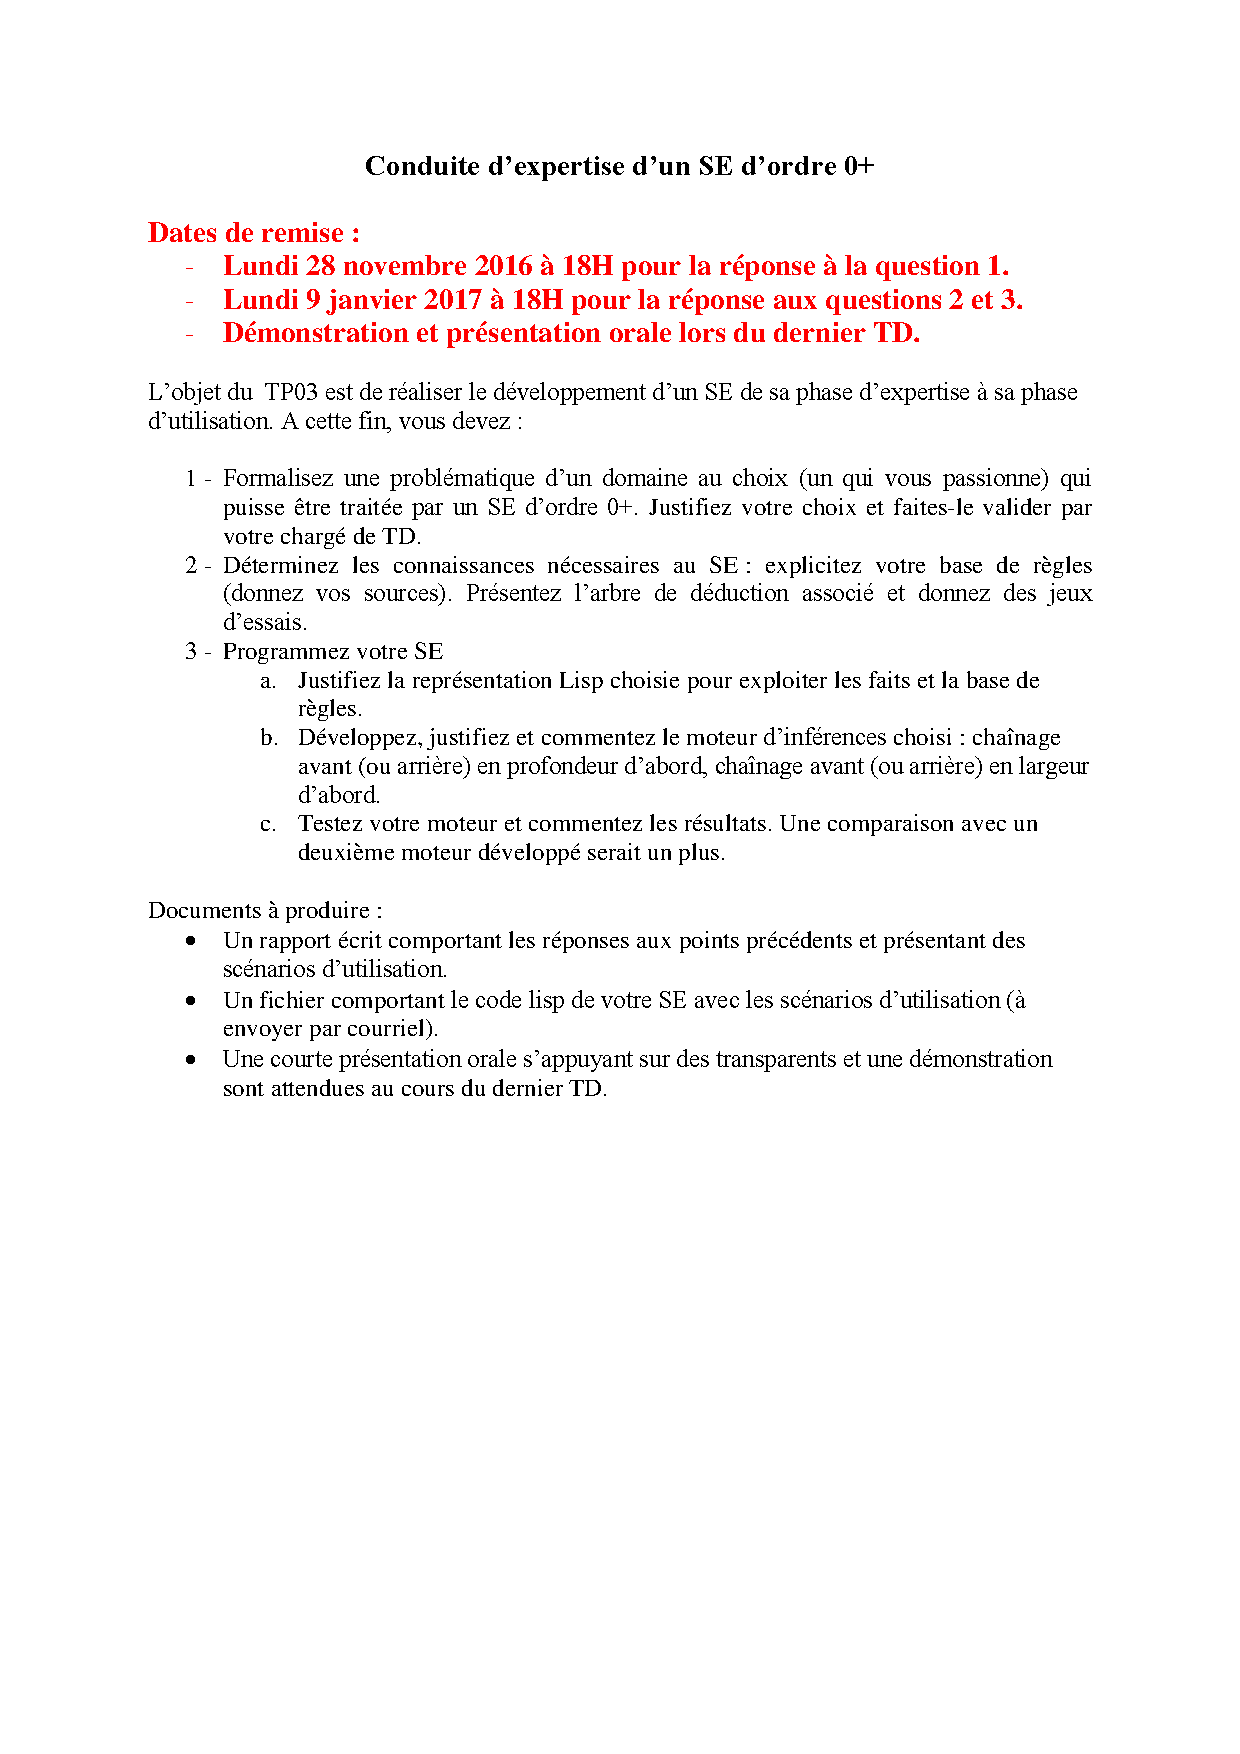
\includepdf[pages=1]{sujet.pdf}
\end{document}
